\documentclass[journal,12pt,twocolumn]{IEEEtran}
%
\usepackage{setspace}
\usepackage{gensymb}
\usepackage{siunitx}
\usepackage{tkz-euclide} 
\usepackage{textcomp}
\usepackage{standalone}
\usetikzlibrary{calc}
\newcommand\hmmax{0}
\newcommand\bmmax{0}

%\doublespacing
\singlespacing

%\usepackage{graphicx}
%\usepackage{amssymb}
%\usepackage{relsize}
\usepackage[cmex10]{amsmath}
%\usepackage{amsthm}
%\interdisplaylinepenalty=2500
%\savesymbol{iint}
%\usepackage{txfonts}
%\restoresymbol{TXF}{iint}
%\usepackage{wasysym}
\usepackage{amsthm}
%\usepackage{iithtlc}
\usepackage{mathrsfs}
\usepackage{txfonts}
\usepackage{stfloats}
\usepackage{bm}
\usepackage{cite}
\usepackage{cases}
\usepackage{subfig}
%\usepackage{xtab}
\usepackage{longtable}
\usepackage{multirow}
%\usepackage{algorithm}
%\usepackage{algpseudocode}
\usepackage{enumitem}
\usepackage{mathtools}
\usepackage{steinmetz}
\usepackage{tikz}
\usepackage{circuitikz}
\usepackage{verbatim}
\usepackage{tfrupee}
\usepackage[breaklinks=true]{hyperref}
%\usepackage{stmaryrd}
\usepackage{tkz-euclide} % loads  TikZ and tkz-base
%\usetkzobj{all}
\usetikzlibrary{calc,math}
\usepackage{listings}
    \usepackage{color}                                            %%
    \usepackage{array}                                            %%
    \usepackage{longtable}                                        %%
    \usepackage{calc}                                             %%
    \usepackage{multirow}                                         %%
    \usepackage{hhline}                                           %%
    \usepackage{ifthen}                                           %%
  %optionally (for landscape tables embedded in another document): %%
    \usepackage{lscape}     
\usepackage{multicol}
\usepackage{chngcntr}
\usepackage{amsmath}
\usepackage{cleveref}
\usepackage{amsmath}
%\usepackage{enumerate}

%\usepackage{wasysym}
%\newcounter{MYtempeqncnt}
\DeclareMathOperator*{\Res}{Res}
%\renewcommand{\baselinestretch}{2}
\renewcommand\thesection{\arabic{section}}
\renewcommand\thesubsection{\thesection.\arabic{subsection}}
\renewcommand\thesubsubsection{\thesubsection.\arabic{subsubsection}}

\renewcommand\thesectiondis{\arabic{section}}
\renewcommand\thesubsectiondis{\thesectiondis.\arabic{subsection}}
\renewcommand\thesubsubsectiondis{\thesubsectiondis.\arabic{subsubsection}}

% correct bad hyphenation here
\hyphenation{op-tical net-works semi-conduc-tor}
\def\inputGnumericTable{}                                 %%

\lstset{
%language=C,
frame=single, 
breaklines=true,
columns=fullflexible
}
%\lstset{
%language=tex,
%frame=single, 
%breaklines=true
%}
\usepackage{graphicx}
\usepackage{pgfplots}

\begin{document}


\newtheorem{theorem}{Theorem}[section]
\newtheorem{problem}{Problem}
\newtheorem{proposition}{Proposition}[section]
\newtheorem{lemma}{Lemma}[section]
\newtheorem{corollary}[theorem]{Corollary}
\newtheorem{example}{Example}[section]
\newtheorem{definition}[problem]{Definition}
%\newtheorem{thm}{Theorem}[section] 
%\newtheorem{defn}[thm]{Definition}
%\newtheorem{algorithm}{Algorithm}[section]
%\newtheorem{cor}{Corollary}
\newcommand{\BEQA}{\begin{eqnarray}}
\newcommand{\EEQA}{\end{eqnarray}}
\newcommand{\define}{\stackrel{\triangle}{=}}
\bibliographystyle{IEEEtran}
%\bibliographystyle{ieeetr}
\providecommand{\mbf}{\mathbf}
\providecommand{\abs}[1]{\ensuremath{\left\vert#1\right\vert}}
\providecommand{\norm}[1]{\ensuremath{\left\lVert#1\right\rVert}}
\providecommand{\mean}[1]{\ensuremath{E\left[ #1 \right]}}
\providecommand{\pr}[1]{\ensuremath{\Pr\left(#1\right)}}
\providecommand{\qfunc}[1]{\ensuremath{Q\left(#1\right)}}
\providecommand{\sbrak}[1]{\ensuremath{{}\left[#1\right]}}
\providecommand{\lsbrak}[1]{\ensuremath{{}\left[#1\right.}}
\providecommand{\rsbrak}[1]{\ensuremath{{}\left.#1\right]}}
\providecommand{\brak}[1]{\ensuremath{\left(#1\right)}}
\providecommand{\lbrak}[1]{\ensuremath{\left(#1\right.}}
\providecommand{\rbrak}[1]{\ensuremath{\left.#1\right)}}
\providecommand{\cbrak}[1]{\ensuremath{\left\{#1\right\}}}
\providecommand{\lcbrak}[1]{\ensuremath{\left\{#1\right.}}
\providecommand{\rcbrak}[1]{\ensuremath{\left.#1\right\}}}
\theoremstyle{remark}
\newtheorem{rem}{Remark}
\newcommand{\sgn}{\mathop{\mathrm{sgn}}}
\providecommand{\res}[1]{\Res\displaylimits_{#1}} 
%\providecommand{\norm}[1]{\lVert#1\rVert}
\providecommand{\mtx}[1]{\mathbf{#1}}
\providecommand{\fourier}{\overset{\mathcal{F}}{ \rightleftharpoons}}
%\providecommand{\hilbert}{\overset{\mathcal{H}}{ \rightleftharpoons}}
\providecommand{\system}{\overset{\mathcal{H}}{ \longleftrightarrow}}
	%\newcommand{\solution}[2]{\textbf{Solution:}{#1}}
\newcommand{\solution}{\noindent \textbf{Solution: }}
\newcommand{\cosec}{\,\text{cosec}\,}
\providecommand{\dec}[2]{\ensuremath{\overset{#1}{\underset{#2}{\gtrless}}}}
\newcommand{\myvec}[1]{\ensuremath{\begin{pmatrix}#1\end{pmatrix}}}
\newcommand{\mydet}[1]{\ensuremath{\begin{vmatrix}#1\end{vmatrix}}}
%\numberwithin{equation}{section}
\numberwithin{equation}{subsection}
%\numberwithin{problem}{section}
%\numberwithin{definition}{section}
\makeatletter
\@addtoreset{figure}{problem}
\makeatother
\let\StandardTheFigure\thefigure
\let\vec\mathbf
%\renewcommand{\thefigure}{\theproblem.\arabic{figure}}
\renewcommand{\thefigure}{\theproblem}
%\setlist[enumerate,1]{before=\renewcommand\theequation{\theenumi.\arabic{equation}}
%\counterwithin{equation}{enumi}
%\renewcommand{\theequation}{\arabic{subsection}.\arabic{equation}}
\def\putbox#1#2#3{\makebox[0in][l]{\makebox[#1][l]{}\raisebox{\baselineskip}[0in][0in]{\raisebox{#2}[0in][0in]{#3}}}}
     \def\rightbox#1{\makebox[0in][r]{#1}}
     \def\centbox#1{\makebox[0in]{#1}}
     \def\topbox#1{\raisebox{-\baselineskip}[0in][0in]{#1}}
\vspace{3cm}
\title{Multiple Outputs}
\maketitle
\newpage
%\tableofcontents
\bigskip
\renewcommand{\thefigure}{\theenumi}
\renewcommand{\thetable}{\theenumi}
\begin{abstract}
This document contains theory involved in curve fitting.
\end{abstract}
\section{\textbf{Objective}}
The objective is first to generate a sinosuidal dataset and then to implement linear regression for multiple outputs.
\section{Generate Dataset}
Create a sinusoidal function of the form
\begin{align}
    y = A\sin{2\pi x} + n(t) \label{eq:1}
\end{align}
n(t) is the random noise that is included in the training set. This set consists of N samples of input data i.e. x expressed as shown below
\begin{align}
    x = \myvec{x_{1}, x_{2}, .., x_{N}}^{T}
\end{align}
which give the corresponding values of y denoted as
\begin{align}
    y = \myvec{y_{1}, y_{2}, .., y_{N}}^{T}
\end{align}
\begin{figure}[!h]
\begin{center}
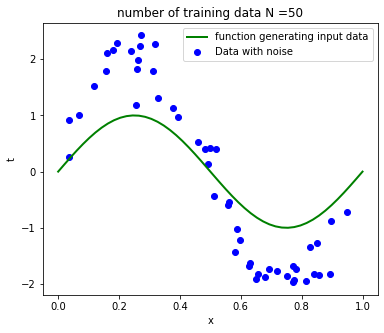
\includegraphics[width=3.4in]{figs/x1.png}
\end{center}
\caption{Sinusoidal Dataset with added noise}
\label{fig:1}
\end{figure}
The Fig \ref{fig:1} is generated by random values of $x_{n}$ for n =1,2,..,N.
where N=50 in the range [0,1].
The corresponding values of y were generated from the Eq \eqref{eq:1}.The first term $A\sin{2\pi x}$ is computed directly and then random noise samples having a normal(Gaussian) distribution are added inorder to get the corresponding values of y.
\begin{lstlisting}
#Generate the sine curve 
import numpy as np
import matplotlib.pyplot as plt
N = 50
np.random.seed(20)
x = np.sort(np.random.rand(N,1),axis=0)
noise = np.random.normal(0,0.3,size=(N,1))
A = 2.5
y = A*np.sin(2*np.pi*x) + noise
plt.scatter(x,y,c='b',marker='o',label='Data with noise')
plt.xlabel('x');plt.ylabel('y')
\end{lstlisting}
The following code generates the input matrix F
\begin{lstlisting}
sk_poly_deg=3
poly_feature = PolynomialFeatures(degree=sk_poly_deg,include_bias=False)
F = poly_feature.fit_transform(x)
\end{lstlisting}
The generated matrix would look like
\begin{align}
    \vec{F}= \myvec{ 1 & x_{0} & x_{0}^2 & \ldots & x_{0}^{N-1} \\
		1 & x_{1} & x_{1}^2 & \ldots & x_{1}^{N-1} \\
		1 & x_{2} & x_{2}^2 & \ldots & x_{2}^{N-1} \\
		\vdots & & \vdots &  & \vdots  \\
		    1 & \ldots & \ldots & \ldots & x_{N}^{N-1} }\label{eq:12}
\end{align}
\section{Multiple Outputs}
In single output Linear regression we only considered target variable t,But in some cases for multiple outputs we can consider more number of target variables.This can be done by using same basis function to model all components of the target vector.
\begin{align}
     y\brak{w,x}= \vec{W}^{T} \phi (x)\\
\end{align}
Where y is a column vector of dimension K,$\vec{W}$ is a M $\times$ K matrix of parameters and $\phi(x)$ is a M dimensional column vector . 
We can maximize the gaussion function by maximum likelihood function and we can do this by considering :  
\begin{align}
    \hat{\vec{W}} = \brak{\vec{\phi}^T\vec{\phi}}^{-1}\vec{\phi}^T\vec{T} \label{eq:13}
\end{align}
if we examine the result for each target variable we have :
\begin{align}
    \vec{w_{k}}=\brak{\vec{\phi}^T\vec{\phi}}^{-1}\vec{\phi}^T\vec{t_{k}}=\vec{\phi}^{-1}\Vec{t_{k}}
\end{align}
we only need to compute a pseudo inverse matrix $\Vec{\phi^{*}}$ which is shared by all the vectors $w_{k}$.This was the theory behind multiple outputs.\\
Now for the implementation purpose the sinusoidal dataset we generated earlier can be easily generated through a direct function of a library provided in python. By using the direct function we are now creating that sinusoidal dataset also considering the target variables t, here we are taking n\textunderscore target=2.Finally after performing the linear regression operation on the data set it will show us two outputs as we considered target variables to be 2.

\begin{lstlisting}
plt.plot(np.linspace(0,1,50),np.sin(2*np.linspace(0,1,50)*np.pi),c='g',linewidth=2,label='function generating input data')
\end{lstlisting} 
Now, we import make\textunderscore regression from sklearn
\begin{lstlisting}
from sklearn.datasets import make_regression
from sklearn.linear_model import LinearRegression
\end{lstlisting}
Creating datasets of sinosuidal form considering target variables=2
\begin{lstlisting}
X, y = make_regression(n_samples=50, n_features=10, n_informative=5, n_targets=2, random_state=1, noise=0.3)
model = LinearRegression()
model.fit(X, y)
\end{lstlisting}
Plot the predicted output
\begin{lstlisting}
plt.plot(x,model.predict(X),'r',label='Plot after LinearRegression for two targets that is Multioutput ')
plt.legend()
plt.show()
\end{lstlisting}
The plot would look like Fig \ref{fig:2}
\begin{figure}[!h]
\begin{center}
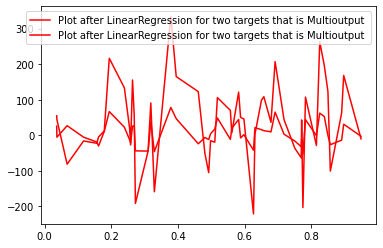
\includegraphics[width=3.4in]{figs/x2.png}
\end{center}
\caption{Linear regression for multiple outputs}
\label{fig:2}
\end{figure}
Python code:
\begin{lstlisting}
https://github.com/sahilsin/EE_IDP/blob/main/Assignment_3/mp.ipynb
\end{lstlisting}
\end{document}